The following section briefly describes what the Giraf project is and its development. 
Giraf is a tool for autistic people with limited verbal communication skills. The project is developed by software engineering students, as part of their bachelor projects. The software engineering students work in small teams and coordinate the work between the teams. The project is in collaboration with the following institutes\cite{GirafWebsite}:

\begin{itemize}
    \item Børnehaven Birken (Kindergarten) \cite{bhBirken}
    \item Egebakken (School) \cite{egebakken}
    \item Enterne (Home for disabled) \cite{enterne}
    \item The speech institute at Aalborg municipality %verify the existence of this institute
    \item Center for Autism and ADHD \cite{center_for_autism}
\end{itemize}

The project started in 2011, and each year, the students continue where the last year students left off.

At the beginning of the project, it was decided to, like previous years, run the project with the \gls{Scrum_principles}. One group was appointed \gls{PO} team and another was appointed Scrum master team. The \gls{PO} team had the responsibility of talking to the customer and making the product backlog. The Scrum master team had the responsibility of deciding and facilitate how the collaboration in the project should run, and whitch guidelines the groups had to follow.

\section{Current state of Giraf}

The Giraf project has produced many different apps over the years; however, with many teams working on the same project throughout multiple years, some problems are bound to have amounted.

These problems come from different ideas, coding styles, and an incomplete mental model of the system, and has resulted in an incoherent structure of the project. Because the groups in 2017 \cite{SW608F18} changed the backend of the system, it left all apps unusable except the Weekplanner, since this is the only app they had time to update to reflect the new backend.

The Weekplanner app is the only app that has received updates in the last couple of years, and with this in mind, the \gls{PO} group also decided to limit our development to the Weekplanner app this year.

The Weekplanner app is a tool for showing autistic people what their plan is for the week. Each day has activities associated with it, ordered in chronologically, each of them represented as a picture also called a pictogram. The state of the app from the start of 2019, can be seen in \autoref{fig:WeekPlannerPicture}.

\begin{figure}[ht]
        \begin{center}
            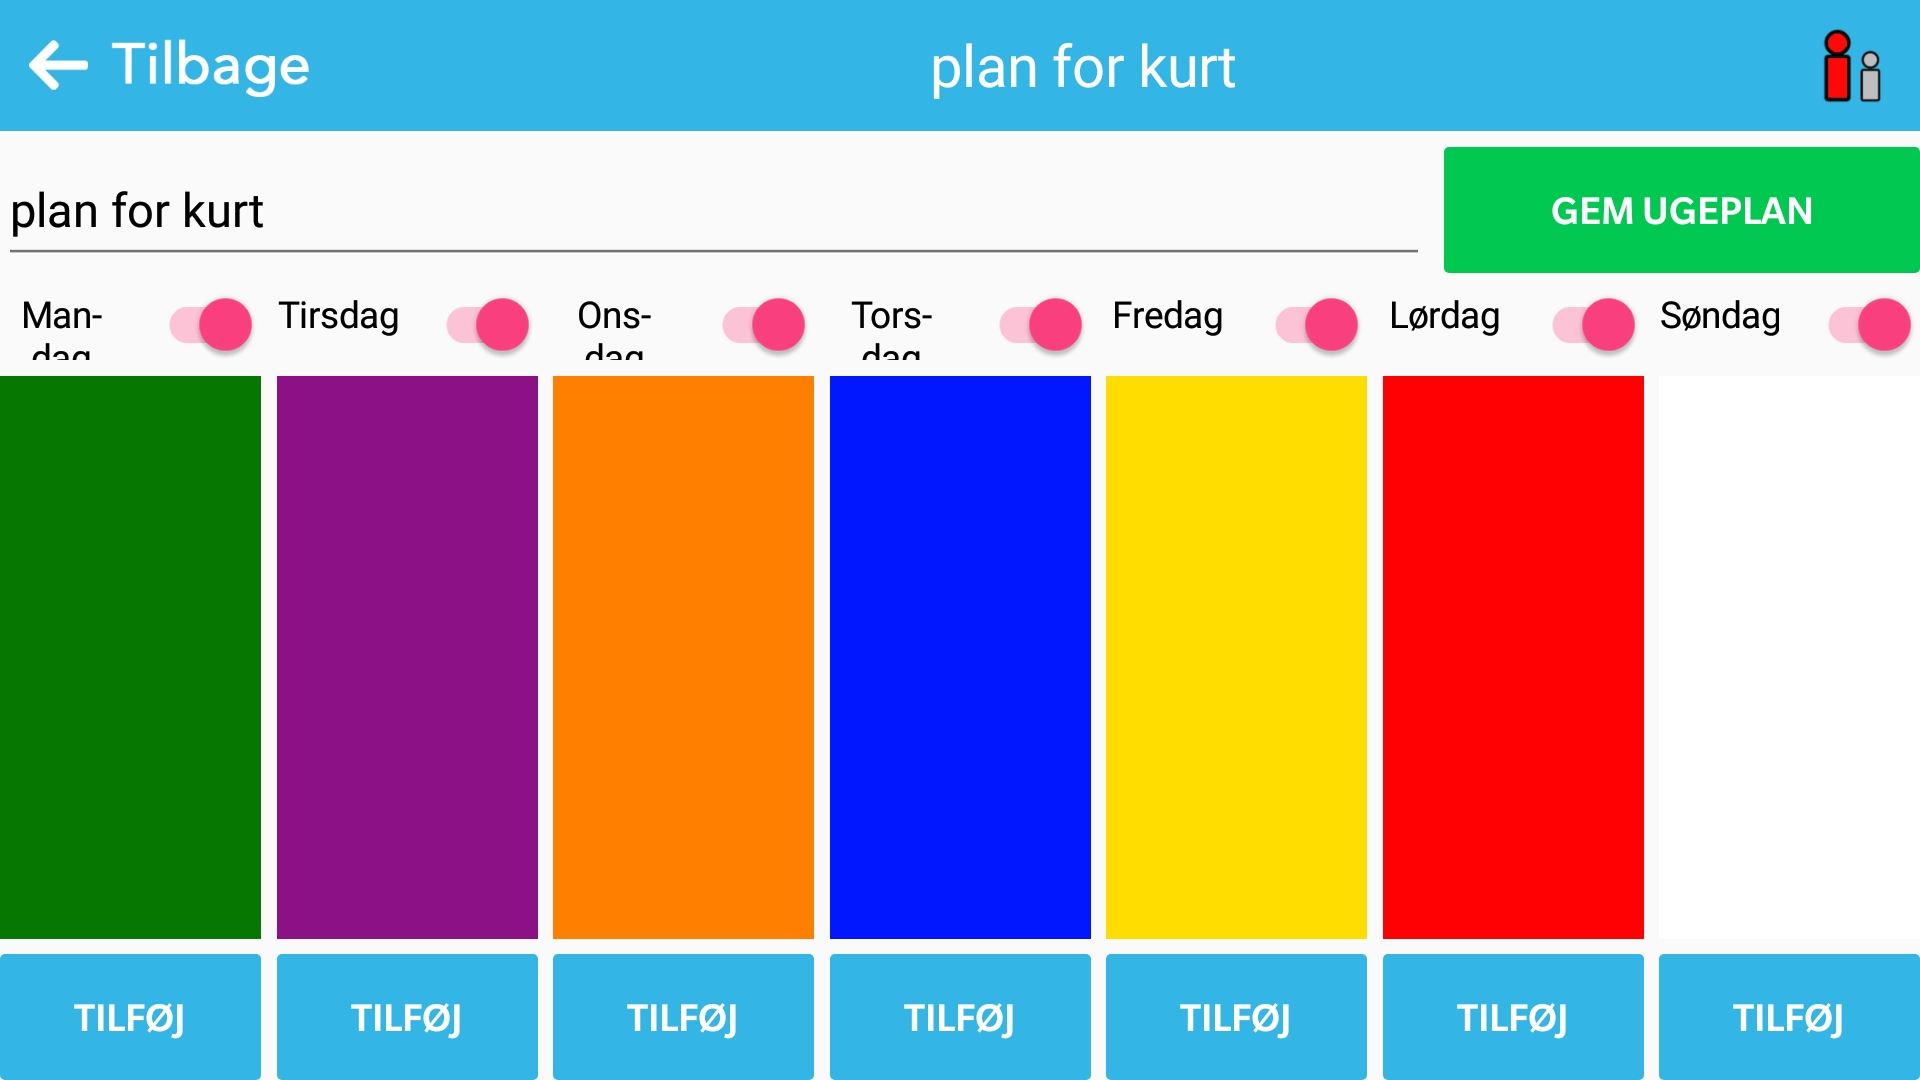
\includegraphics[width=0.95\textwidth]{figures/WeekPlannerPicture}
        \end{center}
        \caption{Weekplanner state at the start of 2019}
        \label{fig:WeekPlannerPicture}
\end{figure}

The Weekplanner app is currently running Xamarin and can run on both Android and IOS devices.
The backend is a .NET Core 2 project that uses traditional MVC. The backend supports all the capabilities of the current Weekplanner app. It exposes a REST-inspired API to the front end.